\documentclass[polish,envcountsect,10pt]{beamer}
    \usepackage[T1]{fontenc}
    \usepackage{fontspec}                 % żeby ustawić czcionkę na systemową (Arial)
    \usepackage[utf8x]{inputenc}
    \usepackage{polski}
    \usepackage{babel}
    \usepackage{hyperref}
    \usepackage{graphicx}
    \usepackage{outlines}
    \usepackage{algorithm2e}

    \newtheorem{mdfn}{Definicja}

    \usetheme{Frankfurt}

    \title{Rozwiązywanie gier}
    \author{Michał Krakowiak}
    \subtitle{Wybrane problemy algorytmiczne i technologiczne, seminarium}
    \date{Gdańsk, 29.10.2019}

\begin{document}
    \frame{\titlepage}
    \section{Wstęp}
        \subsection{Zawartość}
            \begin{frame}
                \frametitle{Zawartość}
                \tableofcontents[pausesections]
            \end{frame}
        \subsection{Tło historyczne}
            \begin{frame}
                \frametitle{Tło historyczne}
                \begin{itemize}
                    \item<1-> 1949, Claude Shannon, komputer a szachy
                    \item<2-> hmmm
                \end{itemize}
            \end{frame}
        \subsection{Definicja gry}
            \begin{frame}
                \frametitle{Czym jest gra?}
                Krótki opis pojęcia gry
            \end{frame}
            \begin{frame}
                \frametitle{Gra w ujęciu kombinatorycznym}
                Właściwości rozważanych gier:
                \begin{itemize}
                    \item<2-> Udział tylko dwóch graczy
                    \item<3-> Przebieg nie zależy od czynników losowych
                    \item<4-> Gracze wykonują ruchy naprzemiennie \textit{(ang. Sequential)}
                    \item<5-> Gracze posiadają pełną wiedzę o stanie gry \textit{(ang. Perfect information)}
                    \item<6-> Gra kończy się po skończonej liczbie ruchów
                    \item<7-> Wygrywa gracz, który wykona ostatni ruch
                \end{itemize}
            \end{frame}
    \section{Klasyfikacja rozwiązań}
        \subsection{Przegląd}
            \begin{frame}
                \frametitle{Klasyfikacja rozwiązań}
                \begin{itemize}
                    \item<1-> Ultra słabe
                    \item<2-> Słabe
                    \item<3-> Mocne
                \end{itemize}
            \end{frame}
        \subsection{Ultra słabe}
            \begin{frame}
                \frametitle{Rozwiązania ultra słabe}
                \begin{itemize}
                    \item<1-> Udowodniono, że gracz wygrywa/przegrywa/remisuje ze startowej pozycji, jeżeli wszyscy grają idealnie \textit{(ang. perfect play)}
                    \item<2-> Przeprowadzony dowód może być niekonstruktywny
                    \item<3-> \textbf{Nie jest wymagane określenie żadnego z ruchów idealnej gry}
                \end{itemize}
            \end{frame}
        \subsection{Słabe}
            \begin{frame}
                \frametitle{Rozwiązania słabe}
                \begin{itemize}
                    \item<1-> Jest znany algorytm, który pozwala jednemu z graczy utrzymać zwycięstwo lub remis od początku gry, niezależnie od ruchów przeciwnika
                    \item<2-> Dzięki podanemu algorytmowi uzyskano przynajmniej jedną \textit{idealną grę} oraz podano dowód, że każdy ruch jest optymalny dla gracza, który go wykonuje                    
                \end{itemize}     
            \end{frame}
        \subsection{Mocne}
            \begin{frame}
                \frametitle{Rozwiązania mocne}
                \begin{itemize}
                    \item<1-> Jest znany algorytm pozwalający uzyskać najlepsze ruchy z każdej pozycji (nawet jeżeli, któryś z graczy popełnił błąd)
                    \item<2-> Częste wykorzystanie metod siłowych \textit{(ang. brute force)} 
                    \item<3-> Dowód może nie być pomocny w zrozumieniu powodów dlaczego dana gra jest rozwiązywalna
                \end{itemize}
            \end{frame}
            \begin{frame}
                \frametitle{Kółko i krzyżyk}
                \begin{figure}[H]
                    \centering
                    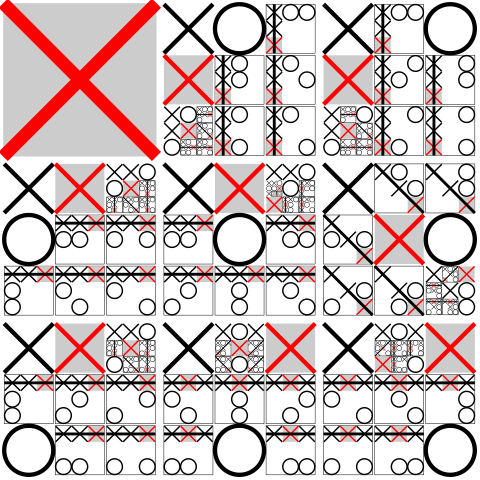
\includegraphics[width=0.55\textwidth,natwidth=480,natheight=480]{images/480px-Tictactoe-X.svg.png}
                    \caption{Optymalna gra dla X}
                \end{figure}
            \end{frame}
        \subsubsection{Kółko i krzyżyk}
            \begin{frame}
                \frametitle{Kółko i krzyżyk}
                \begin{figure}[H]
                    \centering
                    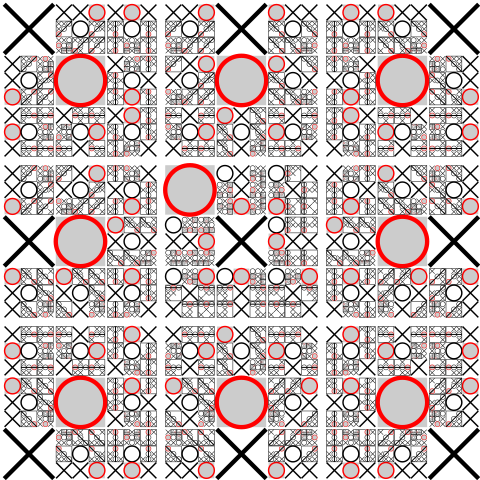
\includegraphics[width=0.55\textwidth,natwidth=480,natheight=480]{images/480px-Tictactoe-O.svg.png}
                    \caption{Optymalna gra dla O}
                \end{figure}
            \end{frame}
        \subsubsection{Nim}
            \begin{frame}
                \frametitle{Nim}                
            \end{frame}
    \section{Szachy}
        \begin{frame}
            \frametitle{Szachy}
            \begin{figure}[]
                \centering
                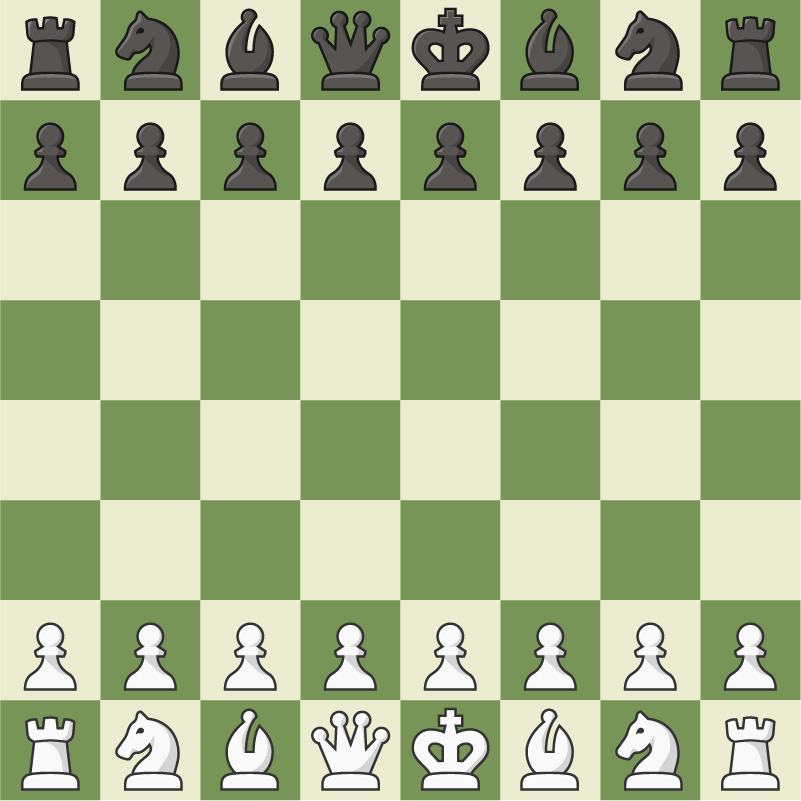
\includegraphics[width=0.55\textwidth]{images/chess.png}
                \caption{Szachy klasyczne}
            \end{figure}
        \end{frame}
        \subsection{Problematyka}
            \begin{frame}
               \frametitle{Problematyka} 
            \end{frame}
        \subsection{Minimax}
            \begin{frame}
                \begin{algorithm}[H]
                    \KwIn{test}
                    \KwOut{test}
                \caption{TEST}
                \end{algorithm}
            \end{frame}
        \subsection{Negamax}
            \begin{frame}
                \frametitle{Negamax}
                %https://en.wikipedia.org/wiki/Negamax
            \end{frame}
        \subsection{Alfa-Beta Pruning}
            \begin{frame}
                \frametitle{Alfa-Beta Pruning}
                %https://en.wikipedia.org/wiki/Alpha–beta_pruning
            \end{frame}
        \subsection{Killer heuristic}
            \begin{frame}
                \frametitle{Killer heuristic}
            \end{frame}
    \section{Literatura}
        \begin{frame}
            \frametitle{Literatura}
            \begin{thebibliography}{9}
                \bibitem{ai_history}Andrey Kurenkov, \emph{A 'Brief' History of Game AI Up To AlphaGo}, \url{https://www.andreykurenkov.com/writing/ai/a-brief-history-of-game-ai/} (data dostępu: 26.10.2019)
                \bibitem{wiki_solved_game}Wikipedia, \emph{Solved game}, \url{https://en.wikipedia.org/wiki/Solved_game} (data dostępu: 26.10.2019)
            \end{thebibliography}
        \end{frame}
\end{document}